\documentclass[10pt,xcolor=table,fleqn]{beamer}

%\usefonttheme{professionalfonts} % using non standard fonts for beamer
\usefonttheme{serif} % default family is serif
%\usepackage{fontspec}
%\setmainfont{Liberation Serif}

\usetheme{Hannover}
\usecolortheme{dolphin}

\usepackage{wasysym}
\usepackage{multirow}
\usepackage{subfigure}
%\usepackage{color, graphicx}
\usepackage{amsthm,amsmath,amsfonts,amssymb}
\usepackage[utf8]{inputenc}
\usepackage{algpseudocode}
\usepackage[portuguese, ruled, vlined, linesnumbered]{algorithm2e}
%\beamertemplatenavigationsymbolsempty
\newcommand{\dtree}[1]{$#1$-d~tree}
\newcommand{\kdtree}{\dtree{k}}
\newcommand{\bsym}[1]{\boldsymbol{#1}}
%\newcommand{\sol}[1]{\boldsymbol{#1}}
\newcommand{\sol}[1]{#1}
\newcommand{\pnt}[1]{pnt(\sol{#1})}
\newcommand{\fsol}[1]{f(\sol{#1})}
\newcommand{\np}{m}
\newcommand{\nphard}{$\mathcal{NP}$-Hard}
\newcommand{\missingI}[1]{}
\newcommand{\missing}[1]{
  \begin{framed}
    {\scriptsize  #1}
  \end{framed}
}
\newcommand{\weight}[1]{w(\sol{#1})}
\newcommand{\obj}[2]{f_{#1}(\sol{#2})}
\newcommand{\bigweight}[1]{w\big(\sol{#1}\big)}
\newcommand{\setIN}{\{1, \ldots, n\}}
\newcommand{\ext}[2]{ext(\sol{#1}, \sol{#2})}
\newcommand{\domLess}[2]{ \sol{#1} \prec \sol{#2} }
%\newcommand{\logicAnd}{ \textrm{ and } }
\newcommand{\logicAnd}{ \land }
\newcommand{\logicOr}{ \lor}
\newcommand{\solSetA}{ Q }
\newcommand{\solSetB}{ R }
\newcommand{\solSett}{ S_* }
\newcommand{\solSet}{ S }
\newcommand{\rord}{\mathcal{O}_{rev}}
\newcommand{\cb}[2]{cb^{#1}(#2)}  % cost-benefit function
\renewcommand{\leq}{\leqslant}
\renewcommand{\geq}{\geqslant}
\newcommand{\floor}[1]{\left \lfloor{#1}\right \rfloor}

% bar graphs configs
\newcommand{\cmpH}{4.0cm}
\newcommand{\cmpW}{7cm}
\newcommand{\legX}{0.45}
\newcommand{\legY}{-0.30}
\newcommand{\scecore}{SCEcr }
\newcommand{\mokp}{MOKP}
\newcommand{\paretoset}{conjunto Pareto}
\newcommand{\paretosetII}{conjunto Pareto-ótimo}
\newcommand{\knapsackdominates}{domina segundo a mochila}

%%% Other Papers Defs Auxiliars %%%
%\newcommand{\dom}[2]{dom(#1, #2)}
\newcommand{\dom}{\underline{\Delta}}
\renewcommand{\ord}{\mathcal{O}}
%\newcommand{\domk}[2]{dom_k(#1, #2)}
\newcommand{\til}[1]{{#1'}}
\newcommand{\rel}{D}
\newcommand{\relk}{\rel_k}
\newcommand{\relki}[1]{\rel_k^{#1}}
\newcommand{\relkargs}[2]{\relk\big(#1, #2\big)}
\newcommand{\relkargsi}[3]{\relki{#1}\big(#2, #3\big)}
\newcommand{\nrel}{p}

\newcommand{\relI}{\rel_k^r}
\newcommand{\relII}{\rel_k^{\dom}}
\newcommand{\relIII}{\rel_k^{b}}

% big bullet
\newcommand{\bbt}{\,\begin{picture}(-1,1)(-1,-2)\circle*{5}\end{picture}\ }


\newcommand{\otitulo}{
  Indexação Multidimensional para Problemas da Mochila Multiobjetivo com Paretos de Alta Cardinalidade}
\author[]{ \textbf{Marcos Daniel Valadão Baroni} }
\date{31 de julho de 2018}

\newtheorem{mydef}{Definição}
\newtheorem{myprop}{Proposição}
\newtheorem{myteo}{Teorema}

\definecolor{defblue}{rgb}{0.2, 0.2, 0.7}
\definecolor{defred}{rgb}{0.6, 0.2, 0.2}
\definecolor{defgreen}{rgb}{0.2, 0.6, 0.2}
\definecolor{defgray}{rgb}{0.6, 0.6, 0.6}

\renewcommand{\emph}{\textbf}
\newcommand{\mytitle}[1]{
  \begin{center}
    \color{defblue}
    { \LARGE #1 }
  \end{center}
}

\newcommand{\badpt}{{\color{defred} \DOWNarrow }}
\newcommand{\medpt}{{\color{defgray} \CIRCLE }}
\newcommand{\goodpt}{{\color{defgreen} \UParrow }}

\begin{document}

\section{Introdução}

\begin{frame}
	\frametitle{Sumário}
	\begin{enumerate}
		\item Introdução
		\item O problema da mochila multiobjetivo (MOKP)
    \item Indexação multidimensional para verificação de dominância
    \item O Algoritmo de Bazgan
		\item O SCE para o MOKP
		\item Experimentos computacionais
		\item Conclusões e trabalhos futuros
	\end{enumerate}
\end{frame}

\begin{frame}
	\frametitle{}
  \begin{block}{Tese}
    \begin{center}
      É possível otimizar a resolução do problema da mochila
      multiobjetivo através da indexação multidimensional das soluções.
    \end{center}
  \end{block}
\end{frame}

\begin{frame}
	\frametitle{Introdução}
  \begin{itemize}
		\item Introdução
		\item O problema da mochila multiobjetivo (MOKP)
		\item Algoritmos para o MOKP
		\item Indexação multidimensional para verificação de dominância
		\item Experimentos computacionais
		\item Conclusões e trabalhos futuros
	\end{itemize}
\end{frame}

\section{O MOKP}

\begin{frame}
	\frametitle{Problemas de Otimização Multiobjetivo}
  \begin{itemize}
    \item{Otimização simultânea de múltiplos objetivos:
    \begin{align*}
      \text{max} ~ f(x) &=
        \big(f_1(x)
        ,f_2(x)
        ,\ldots
        ,f_{\np}(x)\big) \\
      \text{sujeito a} \quad & x \in X
    \end{align*}
    \begin{center}
      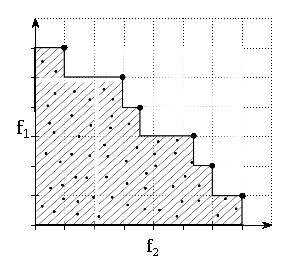
\includegraphics[scale=0.8]{../img/mokp/pareto-def}
    \end{center}
    }
    \item{ Tipicamente mais de uma solução.}
  \end{itemize}
\end{frame}

\begin{frame}
  \frametitle{Problemas de Otimização Multiobjetivo}
  \begin{mydef}[Dominância]
  Diz-se que uma solução $x \in X$
  \emph{domina} uma solução $y \in X$, denotado por $x \dom y$
  se, e somente se, $x$ é ao menos tão boa quanto
  $y$ em todos os objetivos e melhor que $y$ em ao menos um dos objetivos.
  \pause
  Formalmente:
  \begin{equation*}
      x \dom y \iff \left\{
        \begin{array}{l}
            \forall i \in \{1, 2, \ldots, \np\}: f_i(x) \geq f_i(y) ~\text{e}\\
            \exists j \in \{1, 2, \ldots, \np\}: f_j(x) > f_j(y)
    \end{array} \right.
    \label{eq:dom}
  \end{equation*}
  \end{mydef}
  \pause
  \begin{center}
    \vspace*{-4mm}
    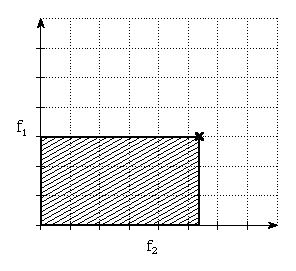
\includegraphics[scale=0.8]{../img/mokp/dom-def}
  \end{center}
\end{frame}

\begin{frame}
  \frametitle{Problemas de Otimização Multiobjetivo}
  \begin{mydef}[Eficiência]
    Uma solução $x \in X$ é dita \emph{eficiente}, denotado por $\text{eff}(x)$,
    se, e somente se, $x$ não é dominada por nenhuma outra solução pertencente a $X$.
    \\ \pause
    Formalmente:
    \begin{displaymath}
      eff(x) \iff \nexists \big(y \in X \wedge y \dom x \big)
    \end{displaymath}
  \end{mydef}
  \pause
  \begin{mydef}[\paretoset{}]
    O conjunto de todas as soluções eficientes de um problema multiobjetivo,
    denotado por $Par(X)$, é chamado de \emph{\paretoset{}} ou \emph{\paretosetII{}}.
    \\ \pause
    Formalmente:
    \begin{displaymath}
      Par(X) = \{ x \in X \;|\; \text{eff}(x)\}
    \end{displaymath}
  \end{mydef}
\end{frame}

\begin{frame}
  \frametitle{Problemas de Otimização Multiobjetivo}
  \vfill
  Resolver um problema multiobjetivo consiste em determinar seu \paretoset{}.
  \vfill \pause
  \begin{center}
    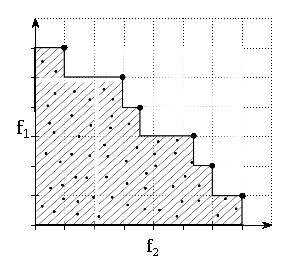
\includegraphics[scale=0.8]{../img/mokp/pareto-def}
  \end{center}
  \vfill
\end{frame}

\begin{frame}
  \frametitle{O Problema da Mochila Multiobjetivo}
  Problema da mochila multiobjetivo (MOKP):
  \begin{itemize}
    \item Generalização do problema da mochila 0-1 (\nphard{});
    \item Bastante estudado pela literatura;
    \item Modela diversos problemas reais:
      \begin{itemize}
        \item Seleção de projetos;
        \item Orçamento de capital;
        \item Planejamento de estoque, etc.
      \end{itemize}
    \item De difícil resolução;
      \begin{itemize}
        \item Especialmente para mais de 2 objetivos.
      \end{itemize}
  \end{itemize}
\end{frame}

\begin{frame}
  \frametitle{O Problema da Mochila Multiobjetivo}
  %Problema da mochila multiobjetivo (MOKP) \\
  \begin{block}{Definição formal:}
    \begin{align*}
      \text{max   } & f(x) =
        \big(f_1(x) ,f_2(x) ,\ldots ,f_{\np}(x)\big) \\
      \text{sujeito a   } & w(x) \leq W \\
      & x \in \{0, 1\}^n\\
      \text{onde} \phantom{mmmmm} \\
      %I_n &= \{1, \ldots, n\}\\
      f_j(x) &= \sum_{i = 1}^n p^j_i x_i \quad j = 1, \ldots, \np\\
      w(x) &= \sum_{i = 1}^n w_i x_i
    \end{align*}
  \end{block}
\end{frame}

\begin{frame}
	\frametitle{O Problema da Mochila Multiobjetivo}
  Exemplo de instância:
  \begin{table}[ht]
    \begin{center}
  \begin{tabular}{|r*{10}{|c}|cc||cc}
  \cline{1-11}
  
    & \multicolumn{10}{c|}{Itens} \\ \cline{1-11}
      & \textbf{1} & \textbf{2} & \textbf{3} & \textbf{4} & \textbf{5} & \textbf{6} & \textbf{7} & \textbf{8} & \textbf{9} & \textbf{10} \\ \cline{1-11}
    \textbf{$\boldsymbol{p^1}$} & 4 & 9 & 3 & 1 & 8 & 7 & 2 & 5 & 6 & 7  \\ \cline{1-11}
    \textbf{$\boldsymbol{p^2}$} & 8 & 4 & 2 & 2 & 3 & 0 & 6 & 8 & 9 & 6  \\ \cline{1-11} \cline{13-14}
    \textbf{$\boldsymbol{w}$}   & 7 & 8 & 5 & 8 & 3 & 5 & 6 & 2 & 4 & 9
        & & \multicolumn{1}{|c|}{$\boldsymbol{W}$}
        & \multicolumn{1}{c|}{28}\\ \cline{1-11} \cline{13-14}
  \end{tabular}
\end{center}
  \end{table}
  \pause
  Conjunto Pareto:
  \begin{table}[ht]
    
\begin{center}
  \begin{tabular}{|c*{10}{|c}||c|c|c|c|}
    \cline{2-14}
    \multicolumn{1}{c|}{}
      & \textbf{1}
      & \textbf{2}
      & \textbf{3}
      & \textbf{4}
      & \textbf{5}
      & \textbf{6}
      & \textbf{7}
      & \textbf{8}
      & \textbf{9}
      & \textbf{10}
      & $\boldsymbol{f_1}$
      & $\boldsymbol{f_2}$
      & $\boldsymbol{w}$ \\ \hline
    \textbf{$\boldsymbol{x_{1}}$} & \bc &     &     &     &     &     & \bc & \bc & \bc & \bc & 24 & 37 & 28 \\ \hline
    \textbf{$\boldsymbol{x_{2}}$} & \bc &     & \bc &     & \bc &     & \bc & \bc & \bc &     & 28 & 36 & 27 \\ \hline
    \textbf{$\boldsymbol{x_{3}}$} & \bc &     &     &     & \bc & \bc & \bc & \bc & \bc &     & 32 & 34 & 27 \\ \hline
    \textbf{$\boldsymbol{x_{4}}$} &     & \bc & \bc &     & \bc &     & \bc & \bc & \bc &     & 33 & 32 & 28 \\ \hline
    \textbf{$\boldsymbol{x_{5}}$} &     & \bc &     &     & \bc & \bc & \bc & \bc & \bc &     & 37 & 30 & 28 \\ \hline
    \textbf{$\boldsymbol{x_{6}}$} &     & \bc & \bc &     & \bc & \bc &     & \bc & \bc &     & 38 & 26 & 27 \\ \hline
  \end{tabular}
\end{center}
  \end{table}
\end{frame}

\begin{frame}
	\frametitle{O Problema da Mochila Multiobjetivo}
  Tamanho do \paretoset{} para instâncias do MOKP com 3 objetivos.
  \begin{center}
   	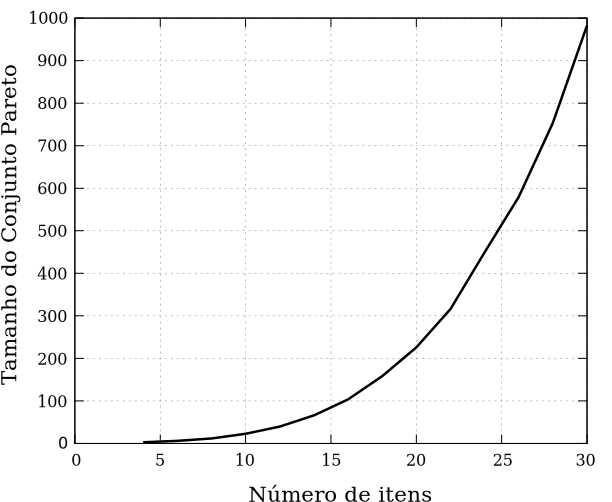
\includegraphics[scale=0.4]{../img/mokp/par-grow-d3}
  \end{center}
\end{frame}

\begin{frame}
  \mytitle{A operação de verificação de dominância}
\end{frame}

\section{A Verificação de Dominância}

\begin{frame}
  \frametitle{A operação de verificação de dominância}
  \only<1-4>{1. Exite alguma solução em $Y$ que \emph{é dominada} por $x$?}
  \begin{center}
    \only<1-2>{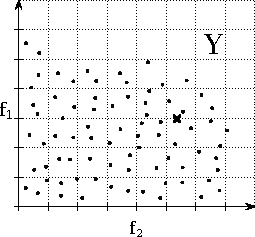
\includegraphics[scale=1.0]{../img/mokp/dom-query-0}}
    \only<3-3>{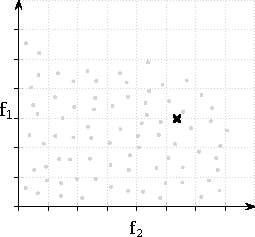
\includegraphics[scale=1.0]{../img/mokp/dom-query-1}}
    \only<4-4>{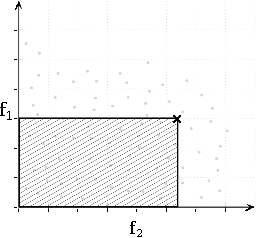
\includegraphics[scale=1.0]{../img/mokp/dom-query-2}
      \\ $\exists(y \in Y)[\; x \dom y \;]$
    }
  \end{center}
\end{frame}

\begin{frame}
  \frametitle{A operação de verificação de dominância}
  1. Exite alguma solução em $Y$ que \emph{é dominada} por $x$?\\
  2. Exite alguma solução em $Y$ que \emph{domina} $x$?
  \begin{center}
    \only<0-1>{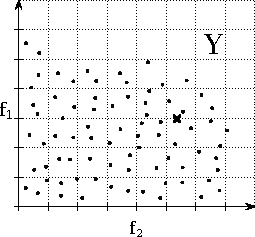
\includegraphics[scale=1.0]{../img/mokp/dom-query-0}}
    \only<2-2>{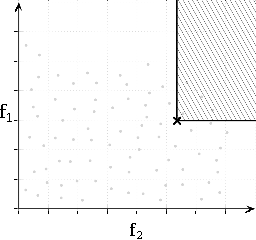
\includegraphics[scale=1.0]{../img/mokp/dom-query-3}
      \\ $\exists(y \in Y)[\; y \dom x \;]$
    }
  \end{center}
\end{frame}

\begin{frame}
  \frametitle{A operação de verificação de dominância}
  A partir de $x$ pode-se definir duas regiões de interesse:\pause
  \begin{center}
    \hfill
    \begin{minipage}[b]{0.42\textwidth}
      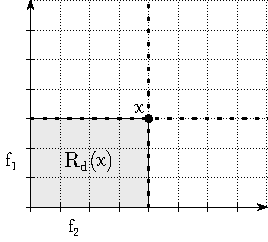
\includegraphics[scale=0.8]{../img/mokp/dom-reg}
      Região \emph{dominada} por $x$.
    \end{minipage}
    \hfill
    \begin{minipage}[b]{0.42\textwidth}
      \only<1-2>{\hspace{6cm}}
      \only<3-3>{
        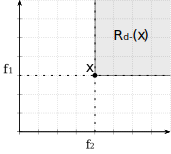
\includegraphics[scale=0.8]{../img/mokp/dom-reg-minus}
        Região que \emph{domina} $x$.
      }
    \end{minipage}
    \hfill
  \end{center}
  \begin{align*}
    &R_d(x) = \big\{y \in \mathbb{R}^\np \;\big|\; y_i \leq f_i(x), i \in \{1, \ldots, \np\}\big\}\\
    \only<3-3>{&R_{d-}(x) = \big\{y \in \mathbb{R}^\np \;\big|\; y_i \geq f_i(x), i \in \{1, \ldots, \np\}\big\}}
  \end{align*}
\end{frame}

\begin{frame}
  \frametitle{Busca de faixa}
  Estruturas de dados para conter soluções:
  \begin{itemize}
    \item{ Lista encadeada (sem indexação)};
    \item{ Árvore AVL (unidimensional)};
    \item{ Árvore KD (multidimensional)}.
  \end{itemize}
\end{frame}

\begin{frame}
  \frametitle{Lista encadeada}
  Lista Encadeada:\\
  \begin{itemize}
    \item{ Implementação simples \goodpt }
    \item{ Pouca utilização de memória \goodpt }
    \item{ Sem indexação -- acesso em tempo linear \badpt }
  \end{itemize}
  \begin{center}
    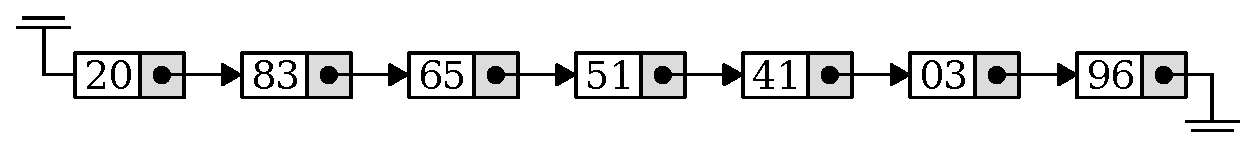
\includegraphics[scale=0.4]{../img/kdt/lst-model}
  \end{center}
\end{frame}

\begin{frame}
  \frametitle{Lista encadeada}
  \begin{center}
    \includegraphics[scale=0.3]{../img/points-query/lst/points}
  \end{center}
\end{frame}

\begin{frame}
  \frametitle{Lista encadeada}
  \begin{center}
    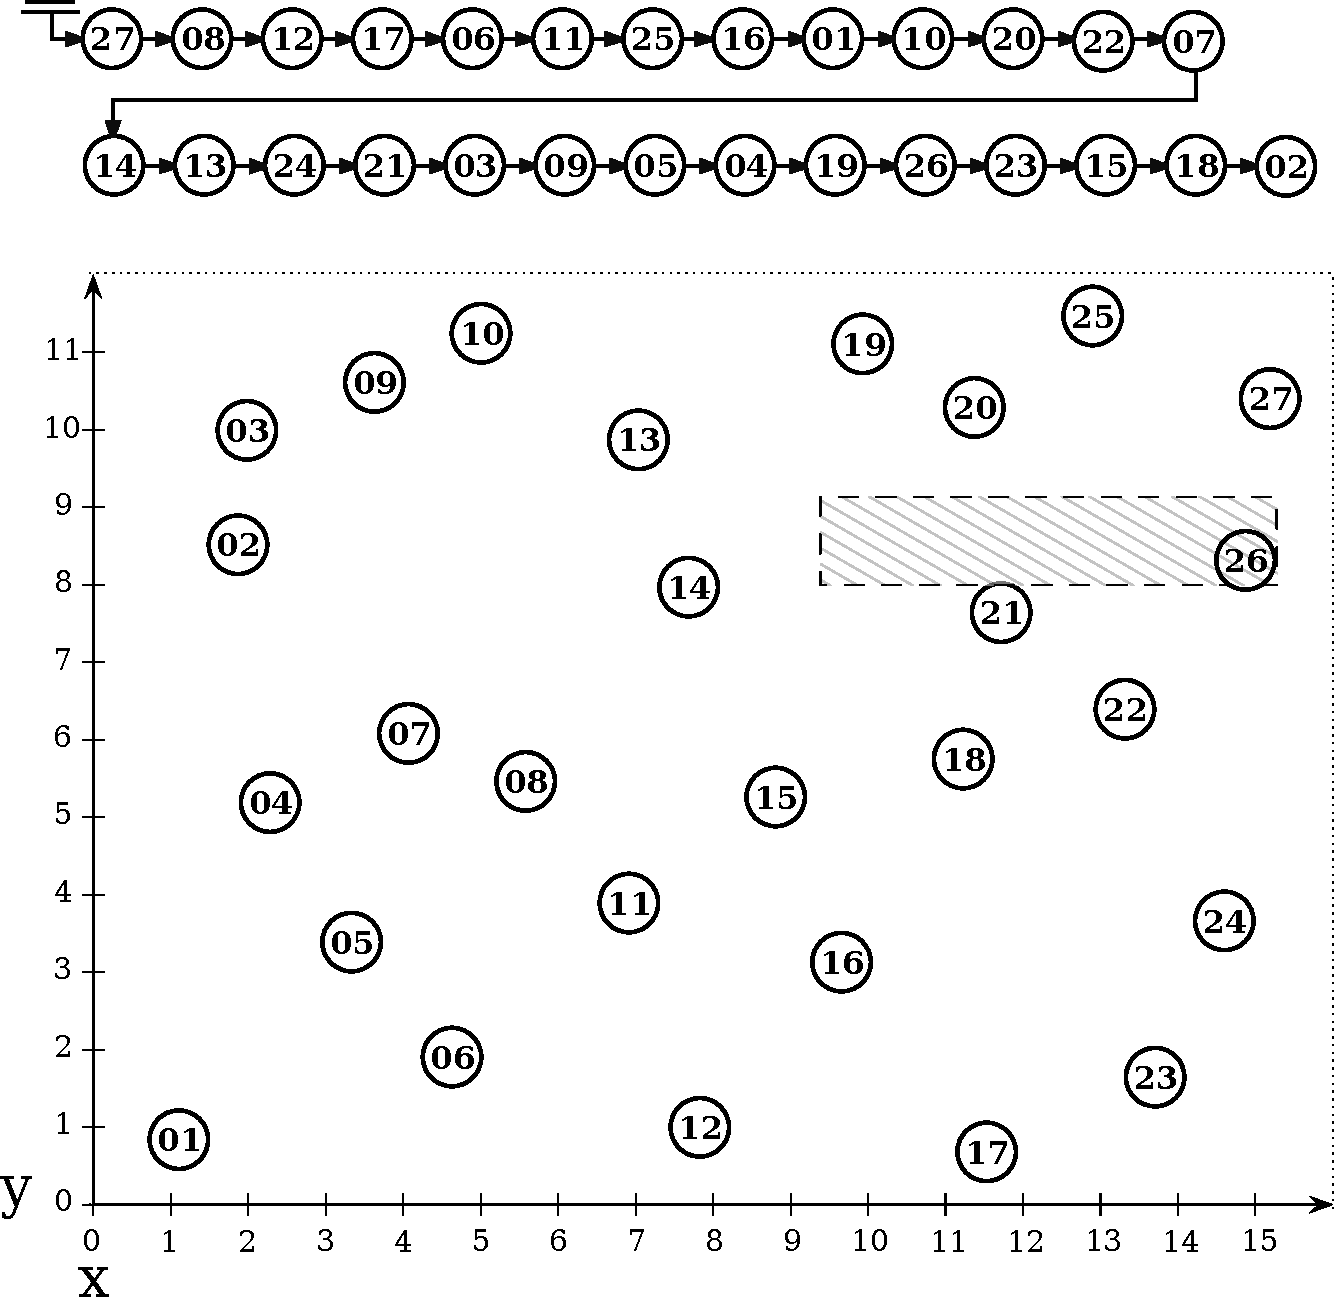
\includegraphics[scale=0.3]{../img/points-query/lst/points-lst-model}
  \end{center}
\end{frame}

\begin{frame}
  \frametitle{Lista encadeada}
  \begin{center}
    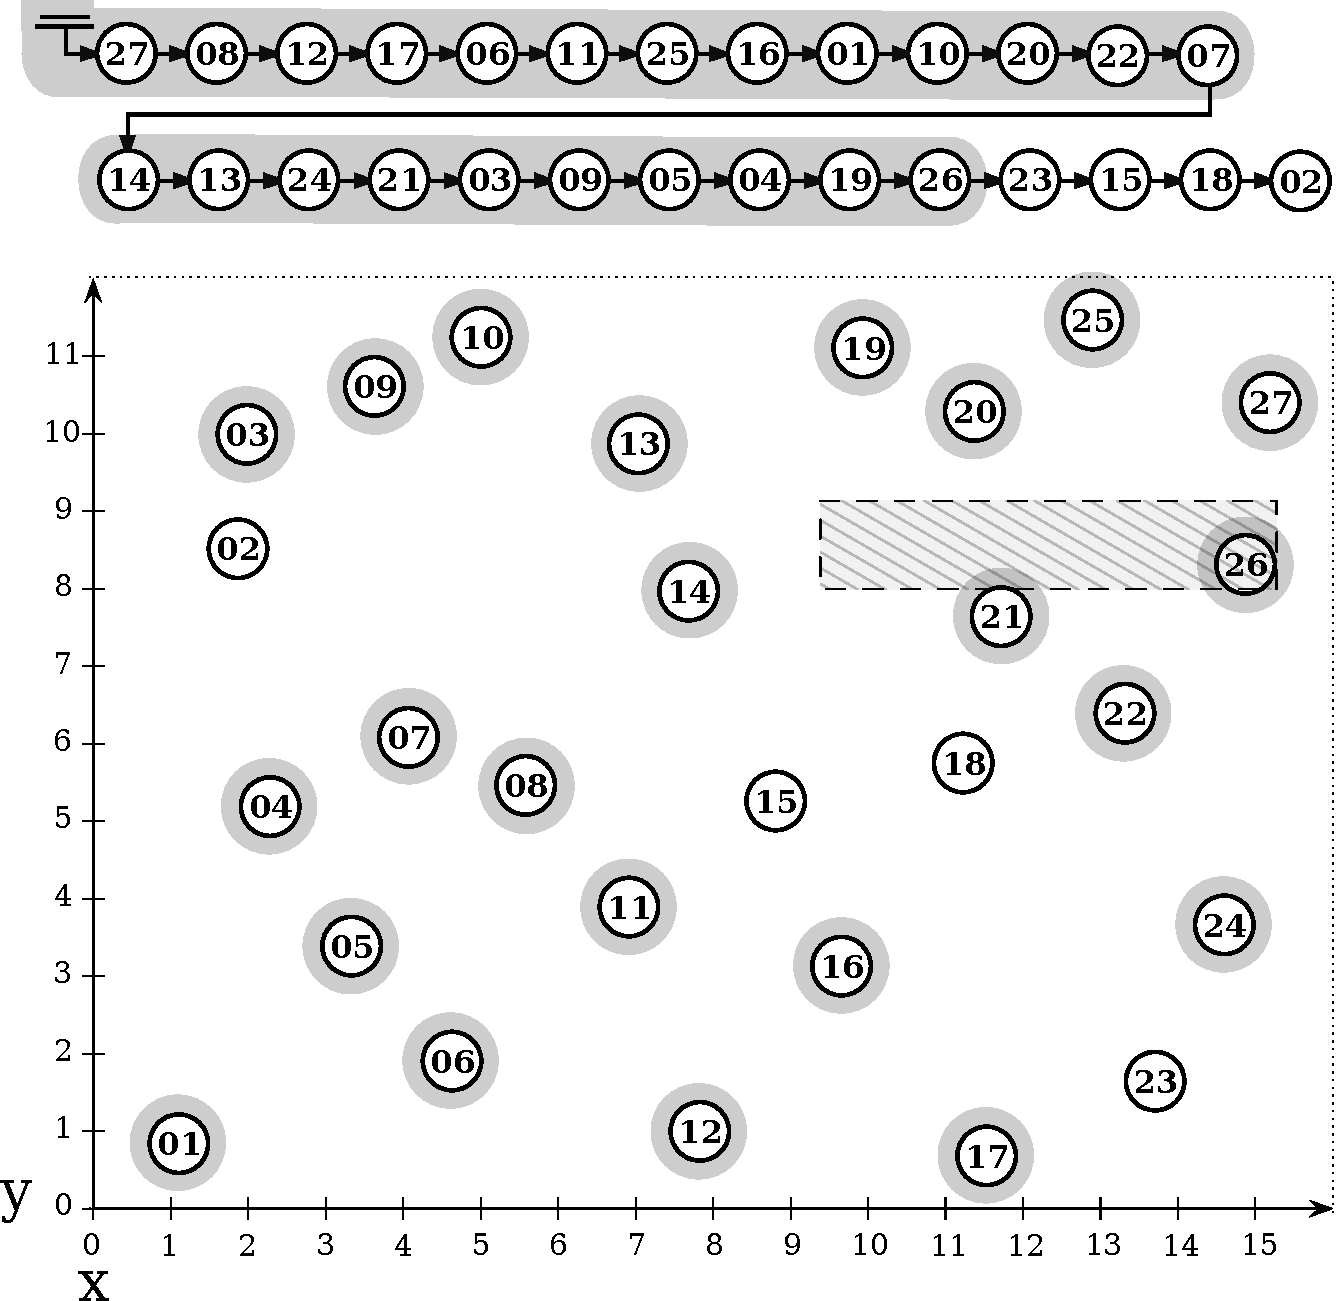
\includegraphics[scale=0.3]{../img/points-query/lst/points-lst-query}
  \end{center}
\end{frame}

\begin{frame}
  \frametitle{Árvore AVL}
  Árvore AVL:\\
  \begin{itemize}
    \item{ Implementação complexa \badpt }
    \item{ Pouca utilização de memória \goodpt }
    \item{ Indexação unidimensional \medpt }
  \end{itemize}
  \pause
  \begin{center}
    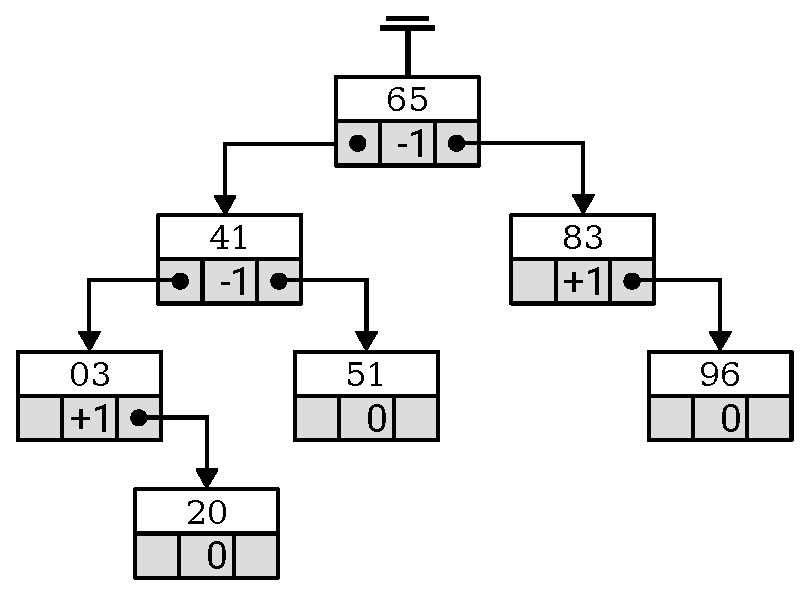
\includegraphics[scale=0.4]{../img/kdt/avl-model}
  \end{center}
\end{frame}

\begin{frame}
  \frametitle{Árvore AVL}
  \begin{center}
    \includegraphics[scale=0.3]{../img/points-query/avl/points}
  \end{center}
\end{frame}

\begin{frame}
  \frametitle{Árvore AVL}
  \begin{center}
    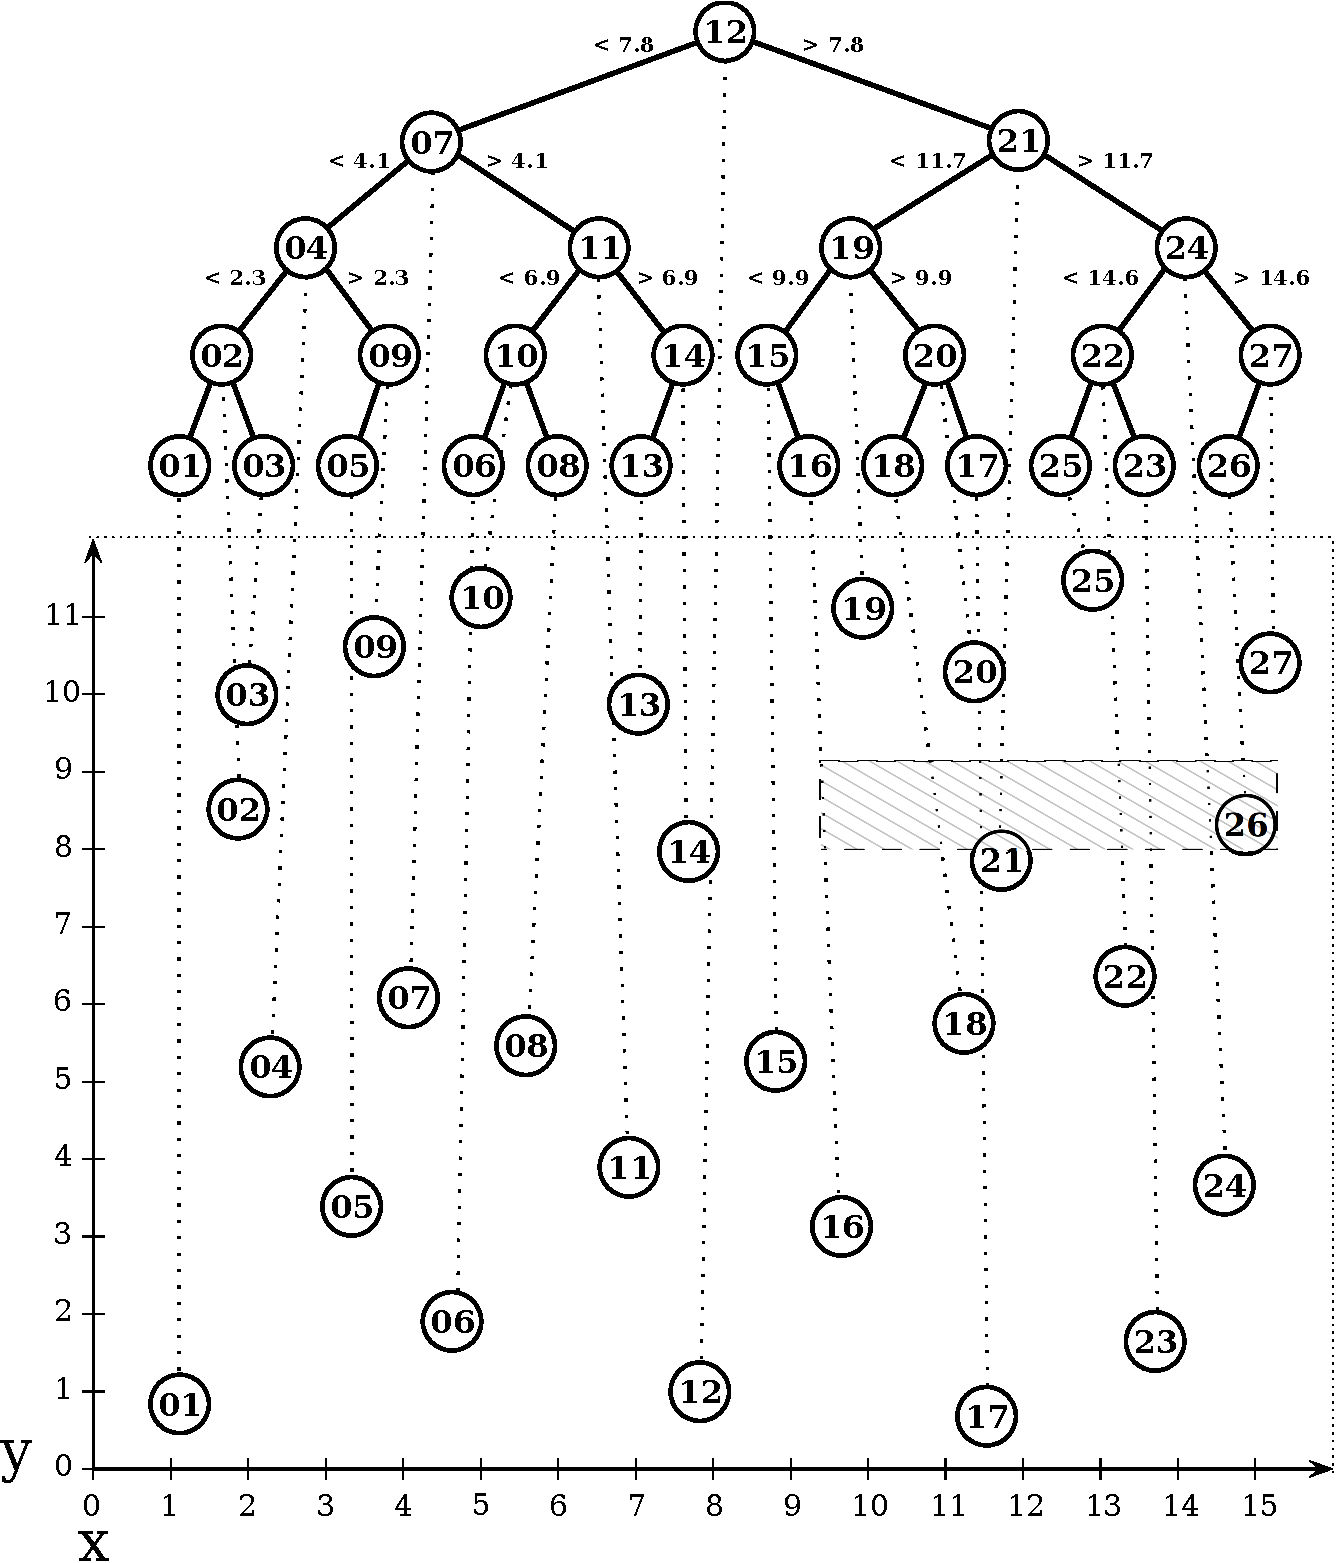
\includegraphics[scale=0.3]{../img/points-query/avl/points-avl-model}
  \end{center}
\end{frame}

\begin{frame}
  \frametitle{Árvore AVL}
  \begin{center}
    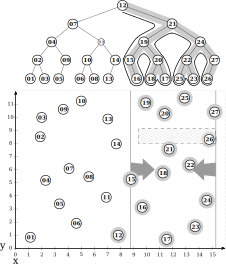
\includegraphics[scale=0.3]{../img/points-query/avl/points-avl-query}
  \end{center}
\end{frame}


\begin{frame}
  \frametitle{Árvore KD}
  Árvore KD:\\
  \begin{itemize}
    \item{ Implementação complexa \badpt }
    \item{ Pouca utilização de memória \goodpt }
    \item{ Indexação multidimensional \goodpt }
  \end{itemize}
  \pause
  \begin{center}
    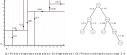
\includegraphics[scale=3.0]{../img/kdt/dom-kd}
  \end{center}
\end{frame}

\begin{frame}
  \frametitle{Árvore KD}
  \begin{center}
    \includegraphics[scale=0.3]{../img/points-query/kdt/points}
  \end{center}
\end{frame}

\begin{frame}
  \frametitle{Árvore KD}
  \begin{center}
    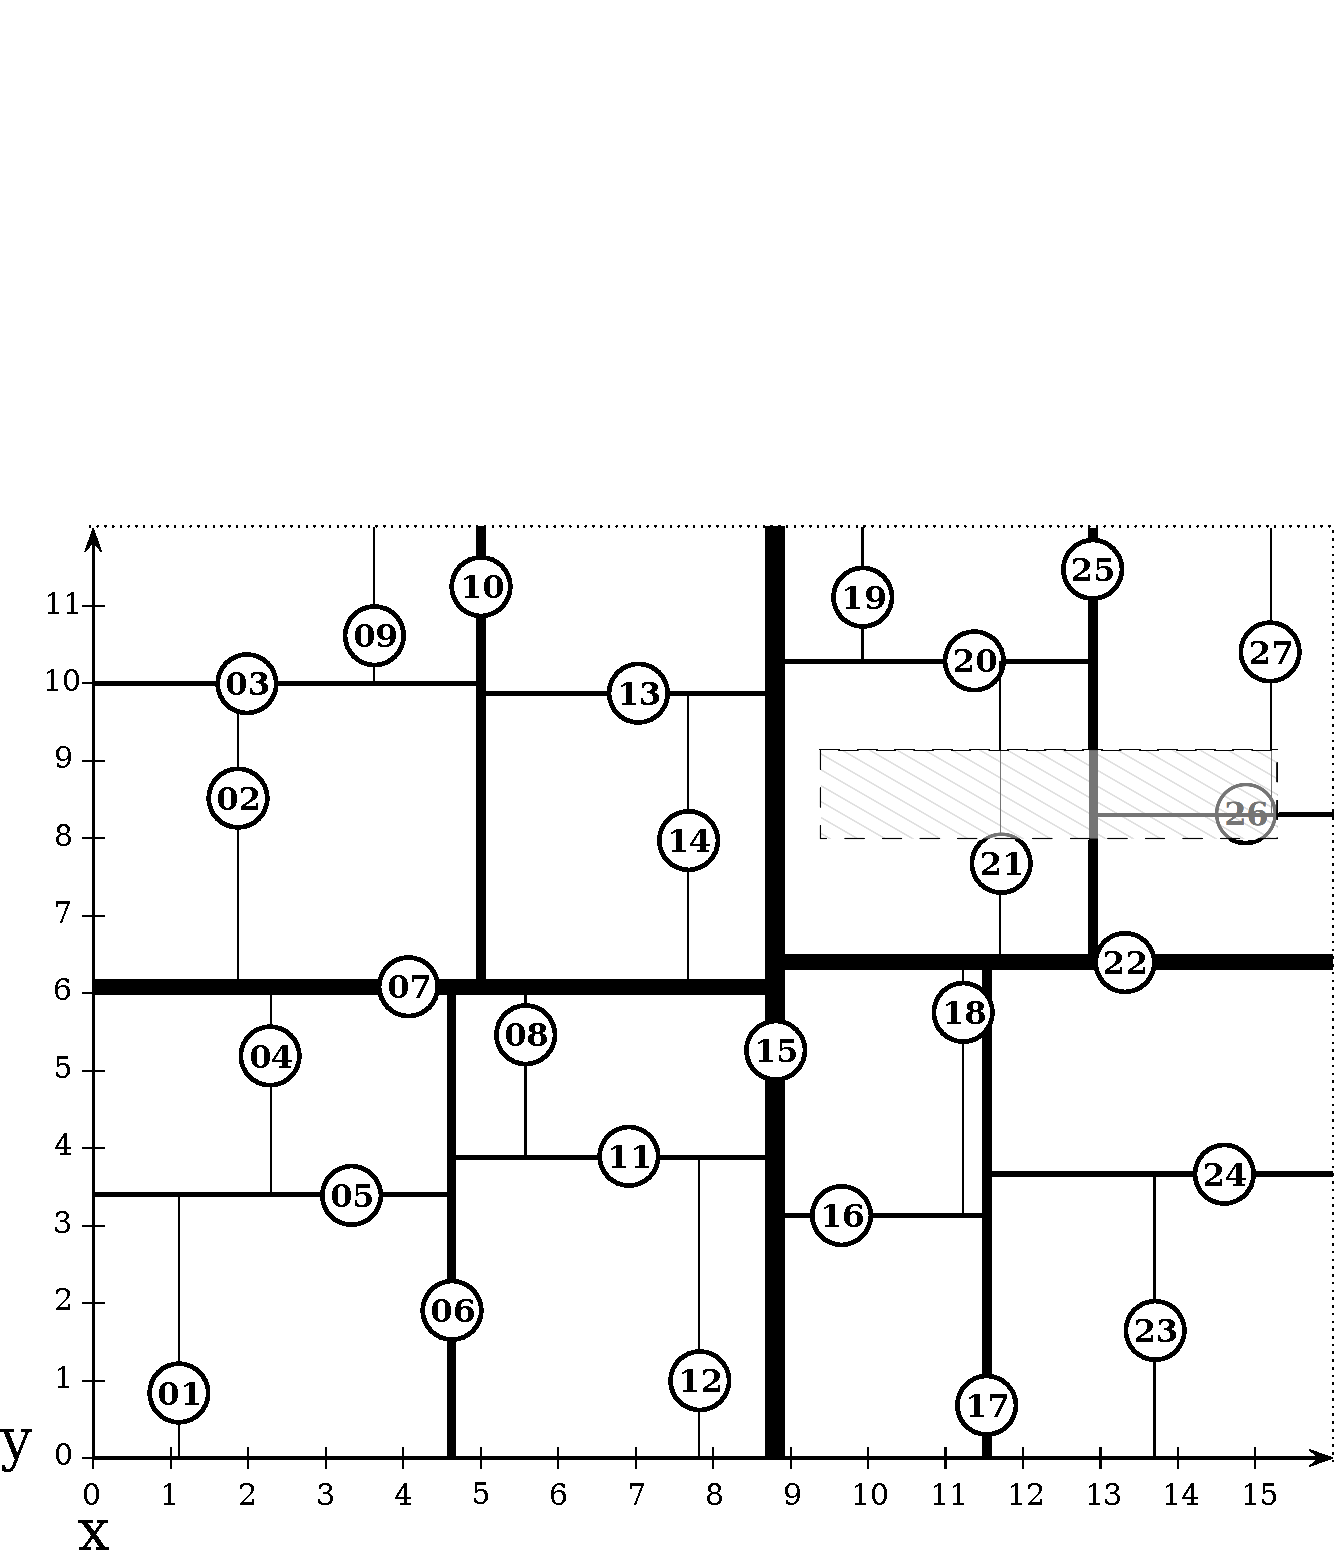
\includegraphics[scale=0.3]{../img/points-query/kdt/points-kdt-model-0}
  \end{center}
\end{frame}

\begin{frame}
  \frametitle{Árvore KD}
  \begin{center}
    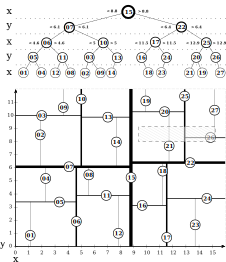
\includegraphics[scale=0.3]{../img/points-query/kdt/points-kdt-model}
  \end{center}
\end{frame}

\begin{frame}
  \frametitle{Árvore KD}
  \begin{center}
    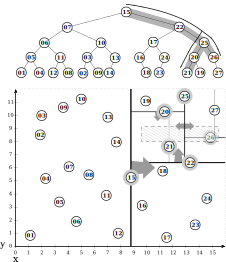
\includegraphics[scale=0.3]{../img/points-query/kdt/points-kdt-query}
  \end{center}
\end{frame}

\section{O Algoritmo de Bazgan}

\begin{frame}
  \mytitle{Algoritmos para o MOKP}
\end{frame}

\begin{frame}
  \begin{block}{Algoritmo Exato}
    \begin{itemize}
      \item Algoritmo de Bazgan -- estado da arte;
    \end{itemize}
  \end{block}
  \begin{block}{Algoritmo Heurístico}
    \begin{itemize}
      \item SCE para o MOKP -- proposta do trabalho;
    \end{itemize}
  \end{block}
\end{frame}

\begin{frame}
	\frametitle{O Algoritmo de Bazgan}
  \begin{itemize}
    \item{ Algoritmo exato de melhor desempenho; }
    \item{ Algoritmo de programação dinâmica -- variação do Nemhauser-Ullmann; }
    \item{ Utiliza 3 dominâncias para redução do conjunto de estados.}
  \end{itemize}
\end{frame}

\begin{frame}
	\frametitle{O Algoritmo de Bazgan}
  \begin{algorithm}[H]
    \footnotesize
    \Kw{$\bsym{p}, \bsym{w}, W$}
\Begin{
  \SetAlgoLined
  $S^0 = \big\{\emptyset\big\}$\;
  \For{$k \gets 1, n$}{
    $S_*^k = S^{k-1} \cup \{\sol{x} \cup k \:|\: \sol{x} \in S^{k-1}\}$\;
    TODO...\;
  }
  $P = \{\sol{x} \:|\: \nexists \sol{a} \in S^n: \dom{a}{x} \;|\; \weight{x} \leq W \}$\;
  \textbf{return} $P$\;
}
    \caption{O algoritmo de Nemhauser e Ullmann para o \mokp.}
  \end{algorithm}
  \pause
  Relações de dominância utilizadas:
  \begin{enumerate}
    \item{ $\rel^r$: Soluções deficientes;}
    \item{ $\rel^{\dom}$: Soluções ``\textit{pesadas}'';}
    \item{ $\rel^{b}$: Soluções não promissoras.}
  \end{enumerate}
\end{frame}

\begin{frame}
	\frametitle{O Algoritmo de Bazgan}
  \begin{block}{1. A relação $\rel^r$:}
    Caso a capacidade residual de uma solução associada a um estado $s_k$
    da iteração $k$ seja maior ou igual à soma dos pesos dos itens restantes,
    o único complemento de $s_k$ que pode resultar
    em uma solução eficiente é o complemento máximo $I = \{k+1, \ldots, n\}$.
  \end{block}
  \pause
  \begin{displaymath}
    s_k \relI s_{\til{k}}
      \Leftrightarrow
      \begin{cases}
        s_{\til{k}} \in S_{k-1}, \\
        s_k = (s_{\til{k}}^1 + p_k^1, \ldots, s_{\til{k}}^\np + p_k^\np, s_{\til{k}}^{\np+1} + w_k), \; \text{e} \\
        s_{\til{k}}^{\np+1} \leq W - \sum_{i=k}^n w_i
      \end{cases}
  \end{displaymath}
\end{frame}

\begin{frame}
	\frametitle{O Algoritmo de Bazgan}
  \begin{block}{2. A relação $\rel^{\dom}$:}
    Generalização para o caso multiobjetivo
    da relação de dominância utilizada no Algoritmo de Nemhauser Ullmann.
  \end{block}
  \pause
  \begin{displaymath}
    s_k \relII s_{\til{k}}
      \Leftrightarrow
      \begin{cases}
        s_k \dom s_{\til{k}} \; & \text{e} \\
        s_k^{\np+1} \leq s_{\til{k}}^{\np+1} \; & \text{se} \; k < n
      \end{cases}
  \end{displaymath}
\end{frame}

\begin{frame}
	\frametitle{O Algoritmo de Bazgan}
  \begin{block}{3. A relação $\rel^{b}$:}\end{block}
  \begin{block}{Limite inferior}
    Vetor objetivo $lb(s) = (lb^1, \ldots, lb^\np)$ onde \\
    \vspace*{2mm}
    \hspace*{4mm}
    $lb^j = s^j + \sum_{i \in J}{p_i^j}$
    \\
    \vspace{2mm}
    para um complemento $J$ qualquer.
  \end{block}
  \pause
  \vspace{5mm}
  \begin{block}{Limite superior}
    Vetor objetivo $u = (u^1, \ldots, u^\np)$ tal que $\forall s_n \in Ext(s_k)$
    tem-se que $u^j \geq s_n^j, \quad j = 1, \ldots, \np$.
  \end{block}
\end{frame}

\begin{frame}
	\frametitle{O Algoritmo de Bazgan}
  \begin{block}{3. A relação $\rel^{b}$:}
    \begin{displaymath}
      s_k \relIII s_{\til{k}}
        \Leftrightarrow
        lb(\sol{u}) \dom ub(\sol{s})
    \end{displaymath}
    \pause
    \vspace{6mm}
    O limite superior utilizado:
    \footnotesize
    \begin{equation*}
      \hspace{-5mm}
      ub^j(s) = s^j + \sum_{i=k+1}^{c_j-1} p_i^j +
        max\left\{ \left\lfloor\overline{W}(s)\frac{p^j_{c_j+1}}{w_{c_j+1}} \right\rfloor ,
         \left\lfloor p^j_{c_j} - \big(w_{c_j} - \overline{W}(s)\big).\frac{p^j_{c_{j-1}}}{w_{c_j-1}}
         \right\rfloor \right\}
    \end{equation*}
    \pause
    \\ \vspace{6mm}
    O limite inferior utilizado (complemento $J$):
    \footnotesize
    \begin{equation*}
      \hspace{-5mm}
      lb^j(s) = s^j + \sum_{i \in J}{p_i^j}, \quad
        \sum_{i \in J}{w_i} \leq \overline{W}(s)
    \end{equation*}
    \vspace{6mm}
  \end{block}
\end{frame}

\begin{frame}
	\frametitle{O Algoritmo de Bazgan}
  \begin{algorithm}[H]
    \footnotesize
    %\Kw{$C_{k-1} = \{ s_{k-1(1)}, \ldots, s_{k-1(r)}\}$
      tal que $s_{k-1(i)} \geq_{lex} s_{k-1(j)} \; \forall i < j (1 \leq i, j \leq r)$}
\Begin{
  $C_k \gets \emptyset; M_k \gets \emptyset; i \gets 1; j \gets 1$\;
  \While{$j \leq r$ \textbf{and} $s_{k-1(1)}^{\np+1} + \sum^n_{l=k}w_l \leq W$}{
    $j \gets j + 1$\;
  }
  \While{$i \leq r$ \textbf{and} $s_{k-1(1)}^{\np+1} + w_k \leq W$}{
    $s_k \gets (s_{k-1(1)}^1 + p_k^1,
      \ldots,
      s_{k-1(1)}^{\np} + p_k^{\np},
      s_{k-1(1)}^{\np+1} + w_k)$\;
    \While{$j \leq r$ \textbf{and} $s_{k-1(j)} \leq_{lex} s_k$}{
      \texttt{MantainNonDominated($s_{k-1(j)}, M_k, C_k$)}; $j \gets j + 1$\;
    }
    \texttt{MantainNonDominated($s_k, M_k, C_k$)}; $i \gets i + 1$\;
  }
  \While{$ j \leq r$}{
    \texttt{MantainNonDominated($s_{k-1(j)}, M_k, C_k$)}; $j \gets j + 1$\;
  }
  \eIf{ k = n }{
    $C_n \gets M_n$\;
  }{
    $F \gets \emptyset$\;
    \For{ $\ord \in \{\ord^{sum}, \ord^{max}\}$}{
      \For{$s_k \in M_k$}{
        Rerotular itens $k+1, \ldots, n$ segundo ordenação $\ord$\;
        $s_n \gets s_k$\;
        \For{$j \gets k + 1, \ldots, n$}{
          \If{$s_n^{\np+1} + w_j \leq W$}{
            $s_n \gets (s_n^1 + p_j^1, \ldots, s_n^{\np} + p_j^{\np}, s_n^{\np+1} + w_j)$\;
          }
        }
        $F \gets \texttt{KeepNonDominated}(s_n, F)$\;
      }
    }
    $i \gets 1; remove \gets true; F \gets \{s_{n(1)}, \ldots, s_{n(h)}\}$\;
    \While{$i \leq c$ \textbf{and} $remove$}{
      Computar limite superior $u$ para $s_{k(i)}$ conforme Equação~\ref{eq:upperb}\;
      $j \gets 1; remove \gets false$\;
      \While{$j \leq h$ \textbf{and} $s_{n(j)} \dom_{lex} u$ \textbf{and} $\neg remove$}{
        \eIf{$s_{n(j)} \dom u$}{
          $remove \gets true$\;
        }{
          $j \gets j + 1$\;
        }
      }
      \If{$remove$}{
        $C_k \gets C_k\backslash \{s_{k(i)}\}; i \gets i + 1$\;
      }
    }
  }
  \textbf{return} $C_k$\;
}

    \begin{algorithmic}[1]
    \Function{BazDP}{$\bsym{p}, \bsym{w}, W$}
    \State $S^0 = [\emptyset ]$
    \For{$k \gets 1, n$}
      \State $S^{k-1} = [\sol{s_1}, \ldots, \sol{s_p}]$
      \State $w_{left} \gets (w_{k} + \ldots + w_n)$
      \State $i \gets min\{i \;| \; \weight{s_i} \geq w_{left}\}$
        \Comment{Deficient solution avoidance}
      \State $j \gets 1$
      \While{ $\bigweight{s^{k-1}_i} < w_{left}$ }
        \State $\ldots$
        \State $i \gets i + 1$
      \EndWhile
      \State $1$
    \EndFor
  %\State $P = \{\sol{x} \:|\: \nexists \sol{a} \in S^n: \dom{a}{x} \}$
  \State \Return $P$
  \EndFunction
\end{algorithmic}

    \caption{Algoritmo Bazgan.}
  \end{algorithm}
  \pause
  \begin{itemize}
    \item{ verificação da condição $u \dom s$ (linha 7);} \pause
    \item{ verificação da condição $lb(u) \dom ub(s)$ (linha 8).}
  \end{itemize}
\end{frame}

\section{O SCE}

\begin{frame}
	\mytitle{O SCE para o MOKP}
\end{frame}

\begin{frame}
	\frametitle{O SCE}
  \begin{itemize}
    \item{ Algoritmo populacional evolutivo; }
    \item{ Evolução simultânea de comunicades independentes; }
    \item{ Utilizado originalmente para resolver problemas hídricos complexos; }
    \item{ \textit{Embaralha} a população em $N$ comunidades (complexos); }
  \end{itemize}
\end{frame}

\begin{frame}
	\mytitle{O SCE}
  \vspace{-5mm}
  \begin{figure}
    \centering
    \hspace{4mm}
    \begin{minipage}[b]{0.36\textwidth}
      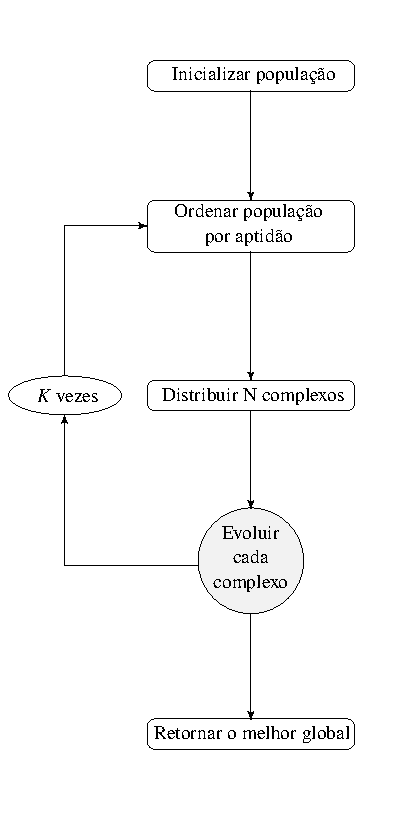
\includegraphics[width=\textwidth]{../img/sce/flow1}
    \end{minipage}
    \hspace{4mm}
    \begin{minipage}[b]{0.36\textwidth}
      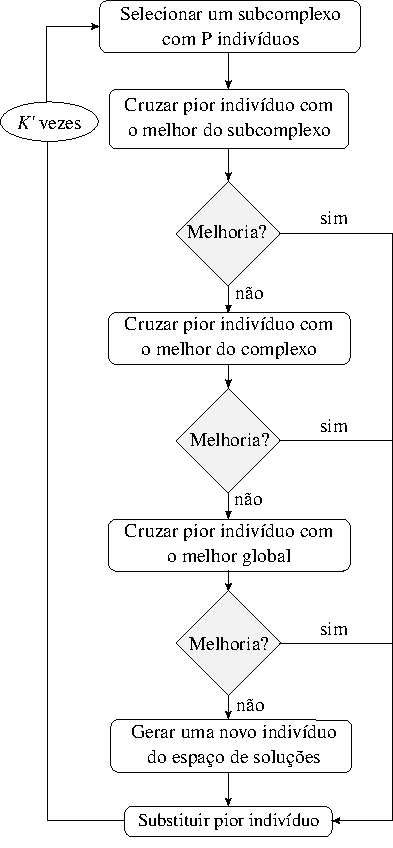
\includegraphics[width=\textwidth]{../img/sce/flow2}
    \end{minipage}
    \hspace{4mm}
  \end{figure}
\end{frame}

\begin{frame}
	\frametitle{O SCE}
  \begin{block}{Adaptação para contexto multiobjetivo:}
    \begin{itemize}
      \item{ Aptidão do indivíduo:
        \only<1>{\\ \phantom{123}}
        \only<2-3>{
        \begin{itemize}
          \item[-] Ordenação em frontes não dominados
        \end{itemize}
        }
      }
      \item{ Construção de \paretoset{} aproximado:
        \only<1-1>{\\ \phantom{123}}
        \only<2-3>{
        \begin{itemize}
          \item[-] Arquivo externo
        \end{itemize}
        }
      }
    \end{itemize}
  \end{block}
  \pause
  \pause
  \begin{block}{Aplicação para o MOKP:}
    \begin{itemize}
      \item{ Construção de solução aleatória;}
      \item{ Procedimento de cruzamento.}
    \end{itemize}
  \end{block}
\end{frame}

\begin{frame}
	\frametitle{O SCE}
  Aptidão do indivíduo: ordenação em frontes não dominados.
  \begin{figure}
    \centering
    \begin{minipage}[t]{0.48\textwidth}
      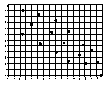
\includegraphics[width=\textwidth]{../img/sce/unrankpop}
      \caption{População sem ordenação.}
      \label{img:unrankpop}
    \end{minipage}
    \hfill
    \begin{minipage}[t]{0.48\textwidth}
      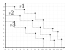
\includegraphics[width=\textwidth]{../img/sce/rankpop}
      \caption{População ordenada em frontes não dominados.}
      \label{img:rankpop}
    \end{minipage}
  \end{figure}
\end{frame}

\begin{frame}
	\frametitle{O SCE}
  Construção de \paretoset{} aproximado: utilização de arquivo externo.
  \vfill
  \begin{algorithm}[H]
    \footnotesize
    \Kw{$A:$ arquivo, $x:$ indivíduo }
\Begin{
  \If{$\nexists (y \in A, y \dom x)$}{
    $A \gets A \cup \{x\}$; \mycomment[1.7cm]{Inclusão de $x$ no arquivo}
    $A \gets A \backslash \{z \in A \;|\; x \dom z\}$; \mycomment{Remoção das soluções dominadas por $x$}
  }
  \textbf{return} $A$\;
}
    \caption{Procedimento de atualização de arquivo, dada uma nova solução.}
    \label{alg:archupdate}
  \end{algorithm}
\end{frame}

\begin{frame}
	\frametitle{O SCE}
  \begin{algorithm}[H]
    \scriptsize
    \Begin{
  Inicializar população de $N*M$ indivíduos gerados aleatoriamente\;
  Classificar população em frontes não dominados \only<2>{{\color{defred} \LEFTarrow}}\;
  Selecionar o 1º fronte para compor arquivo externo\;
  \For{$ k \leftarrow 1:K$}{
    Ordenar população por aptidão (desempate por hipervolume)\;
    Distribuir população em $M$ complexos\;
    \For{$i \leftarrow 1:N$}{
      \For{$k' \leftarrow 1:K'$}{
        Selecionar subcomplexo com $P$ indivíduos retirados do $i$-ésimo complexo\;
        Evoluir pior indivíduo do subcomplexo gerando um novo indivíduo \only<2>{{\color{defred} \LEFTarrow}}\;
      }
    }
    Classificar toda a população (nova e antiga) em frontes não dominados \only<2>{{\color{defred} \LEFTarrow}}\;
    Propor atualização do arquivo utilizando as soluções do 1º fronte $F_1$ \only<2>{{\color{defred} \LEFTarrow}}\;
    Selecionar população;
  }
  \textbf{return} Arquivo externo\;
}

    \caption{Algoritmo SCE adaptado para o MOKP.}
  \end{algorithm}
  \pause
  \begin{itemize}
    \small
    \item{Classificar a população em frontes não dominados (linhas 3 e 12);}
    \item{Verificar se o indivíduo teve aptidão melhorada (linha 11);}
    \item{Atualização do arquivo, dada uma nova solução (linha 13).}
  \end{itemize}
\end{frame}

\section{Experimentos}

\begin{frame}
	\mytitle{Experimentos Computacionais}
\end{frame}

\begin{frame}
	\frametitle{Experimentos Computacionais}
  \framesubtitle{Abordagem Exata}
  Instâncias bi-objetivo divididas em 4 tipos:
  \vspace{3mm}
  \begin{enumerate}
    \item[A)] Aleatórias: $
      p^j_i \in [1, 1000],
      w_i \in [1,1000]$.
    \vspace{3mm}
    \item[B)] Não-conflitantes: $
      p^1_i \in [111, 1000],
      p^2_i \in [p^1_i - 100, p^1_i + 100],
      w_i \in [1,1000]$.
    \vspace{3mm}
    \item[C)] Conflitantes: $
      p^1_i \in [1, 1000],
      p^2_i \in [max\{900-p^1_i;1\}, min\{1100-p^1_i, 1000\}],
      w_i \in [1,1000]$.
    \vspace{3mm}
    \item[D)] Conflitantes com pesos correlacionados: $
      p^1_i \in [1, 1000],
      p^2_i \in [max\{900-p^1_i;1\}, min\{1100-p^1_i, 1000\}],
      w_i \in [p^1_i+p^2_i-200, p^1_i+p^2_i+200]$.
  \end{enumerate}
\end{frame}

\begin{frame}
  \frametitle{Experimentos Computacionais}
  \framesubtitle{Abordagem Exata}
  Instâncias $3$-objetivo divididas em 4 tipos:
  \begin{enumerate}
    \item[A)] Aleatórias: $
      p^j_i \in [1, 1000]
      w_i \in [1,1000]$
    \vspace{3mm}
    \item[B)] Não-conflitantes: $
      p^1_i \in [111, 1000],
      p^2_i \in [p^1_i - 100, p^1_i + 100],
      p^3_i \in [p^1_i - 100, p^1_i + 100],
      w_i \in [1,1000]$.
    \vspace{3mm}
    \item[C)] Conflitantes: $
      p^1_i \in [1, 1000], \;
      p^2_i \in [1, 1001 - p^1_i]
      p^3_i \in [max\{900-p^1_i-p^2_i;1\}, min\{1100-p^1_i-p^2_i, 1001-p^1_i\}]
      w_i \in [1,1000]$.
    \vspace{3mm}
    \item[D)] Conflitantes com pesos correlacionados: $
      p^1_i \in [1, 1000]
      p^2_i \in [1, 1001 - p^1_i]
      p^3_i \in [max\{900-p^1_i-p^2_i;1\}, min\{1100-p^1_i-p^2_i, 1001-p^1_i\}]
      w_i \in [p^1_i+p^2_i+p^3_i-200, p^1_i+p^2_i+p^3_i+200]$.
  \end{enumerate}
\end{frame}

\begin{frame}
  \frametitle{Experimentos Computacionais}
  \framesubtitle{Abordagem Exata}
  Tempo computacional médio do algoritmo Bazgan para instâncias bi-objetivo:
  \scriptsize
  \begin{table}[h]
    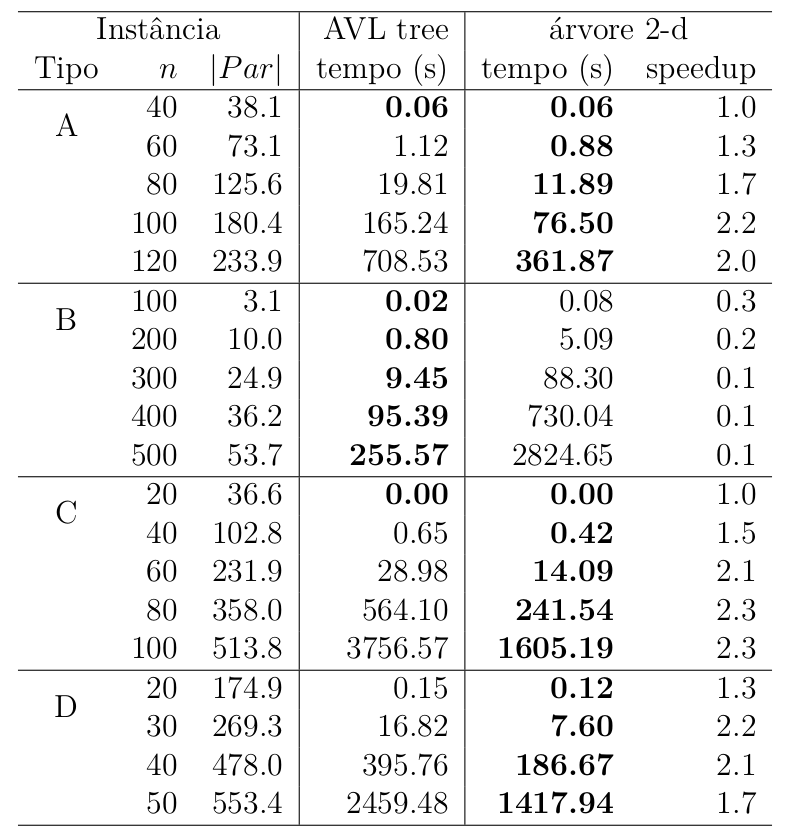
\includegraphics[scale=0.3]{../tab/cpu2dim}
  \end{table}
\end{frame}

\begin{frame}
  \frametitle{Experimentos Computacionais}
  \framesubtitle{Abordagem Exata}
  Número de avaliações médio do algoritmo Bazgan para instâncias bi-objetivo:
  \begin{figure}[H]
    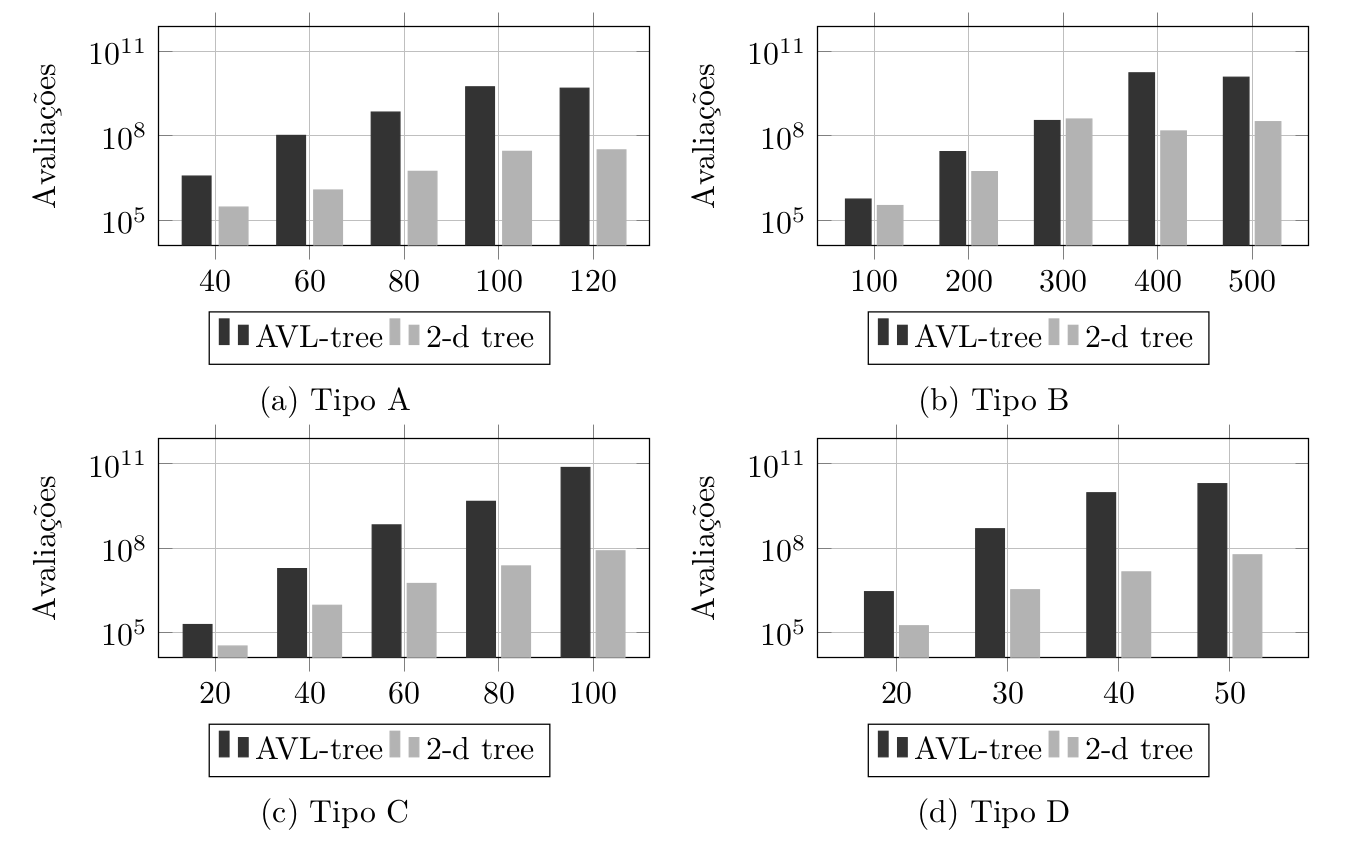
\includegraphics[scale=0.3]{../tab/cmp/2dim}
  \end{figure}
\end{frame}

\begin{frame}
  \frametitle{Experimentos Computacionais}
  \framesubtitle{Abordagem Exata}
  Tempo computacional médio do algoritmo Bazgan para instâncias $3$-objetivo:
  \scriptsize
  \begin{table}[h]
    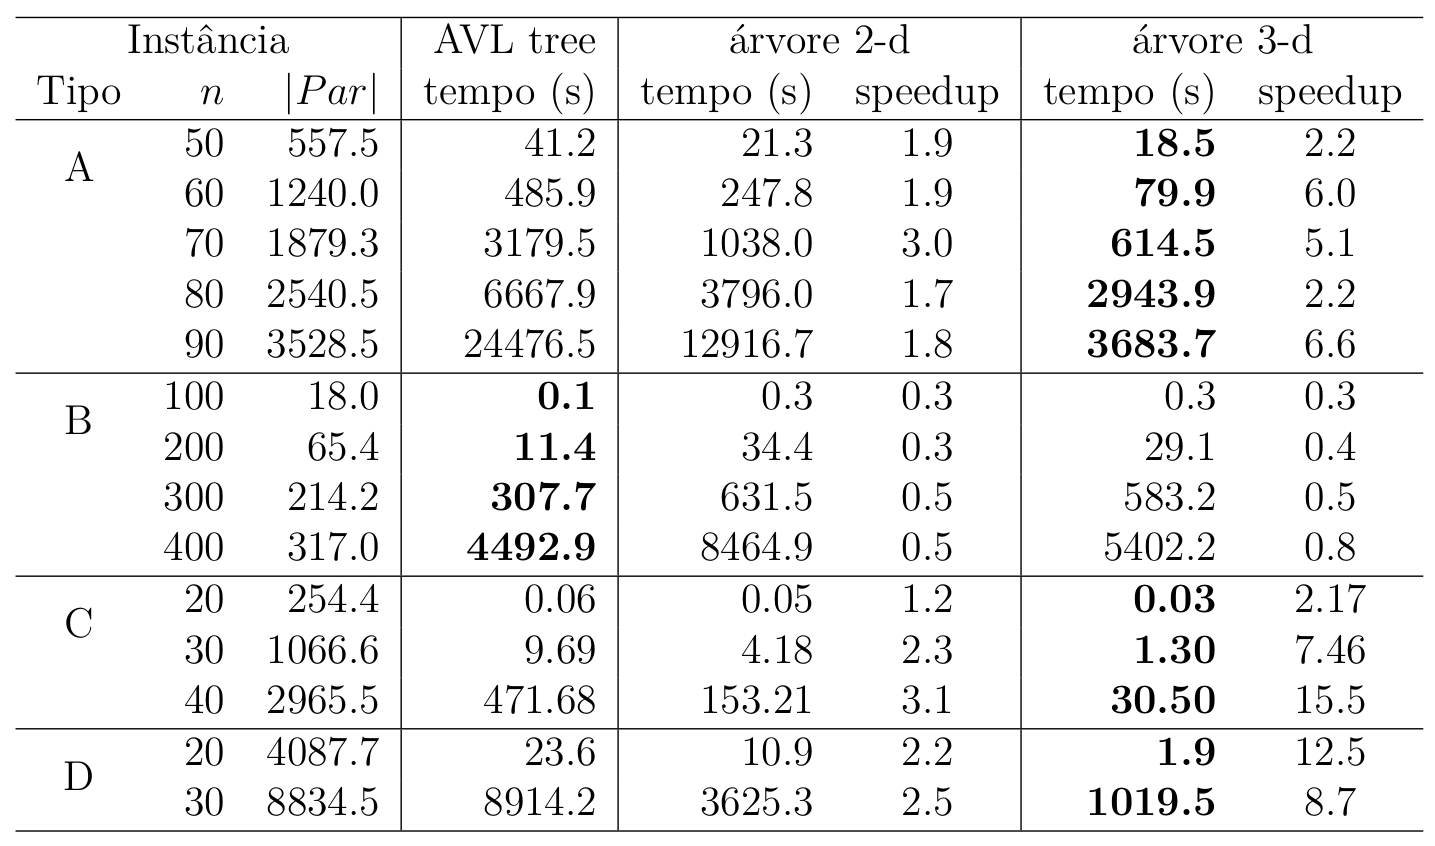
\includegraphics[scale=0.25]{../tab/cpu3dim}
  \end{table}
\end{frame}

\begin{frame}
  \frametitle{Experimentos Computacionais}
  \framesubtitle{Abordagem Exata}
  Número de avaliações médio do algoritmo Bazgan para instâncias $3$-objetivo:
  \begin{figure}[H]
    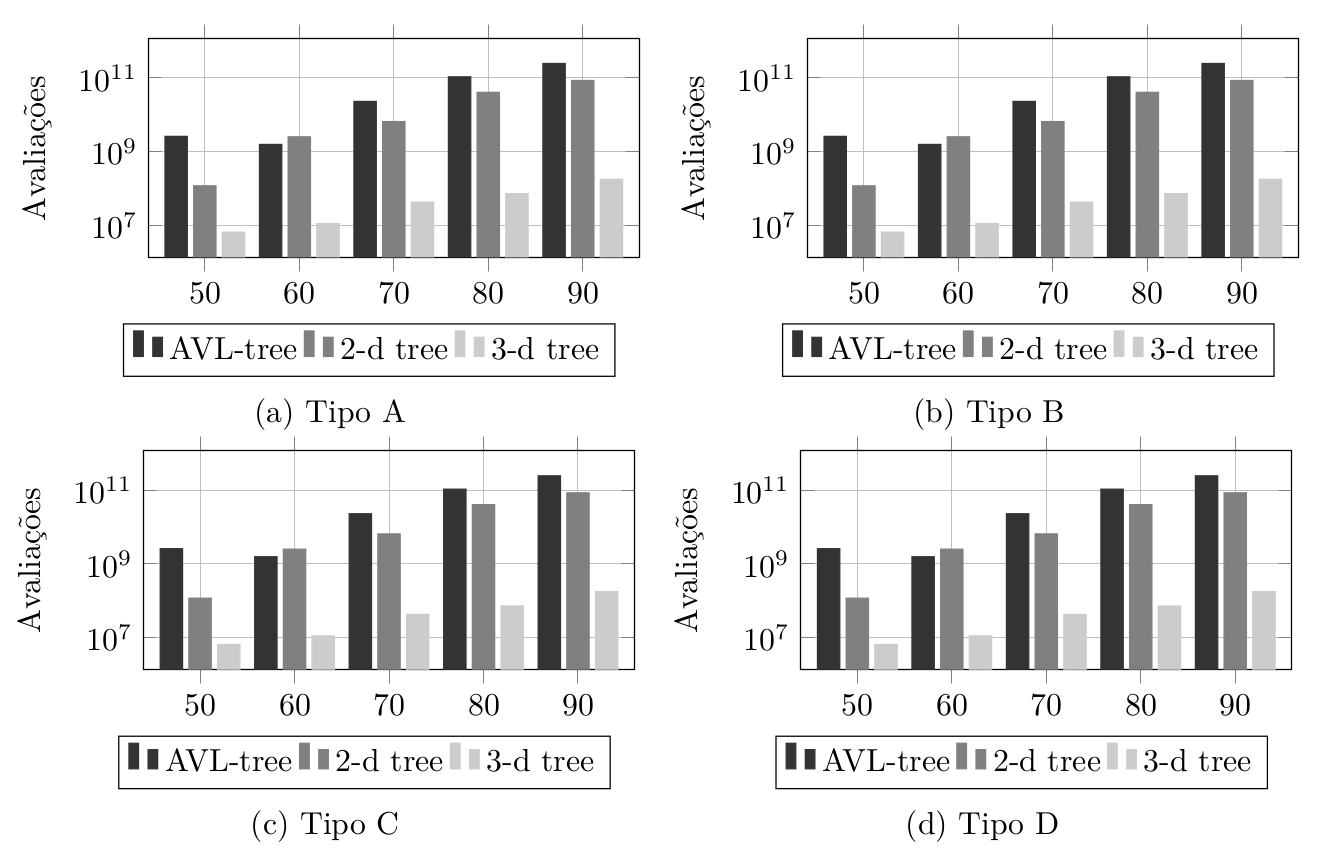
\includegraphics[scale=0.3]{../tab/cmp/3dim}
  \end{figure}
\end{frame}

\begin{frame}
  \frametitle{Experimentos Computacionais}
  \framesubtitle{Abordagem Heurística}
  Valores de parâmetros utilizados no algoritmo SCE:
  \begin{table}[H]
    \small
    \centering
    \begin{tabular}{c|r|p{65mm}}
\hline
  Parâmetro
   & Valor
   & \multicolumn{1}{c}{Descrição} \\ \hline
  N  &  30    & Número de complexos \\ \hline
  M  &  30    & Número de indivíduos em cada complexo\\ \hline
  P  &   5    & Número de indivíduos em cada subcomplexo\\ \hline
  K  & 400    & Número de iterações\\ \hline
  K' &  30    & Número de iterações aplicados a cada evolução de complexo\\ \hline
  c  & $n/20$ & Número de genes carregados no procedimento de cruzamento\\ \hline
\end{tabular}

  \end{table}
\end{frame}

\begin{frame}
  \frametitle{Experimentos Computacionais}
  \framesubtitle{Abordagem Heurística}
  Métrica para avaliação de qualidade de Pareto: hiper-volume.
  \vfill
  Exemplo de conjunto Pareto bi-objetivo possuindo 18 unidades hiper-volume (área):
  \begin{figure}
    \centering
    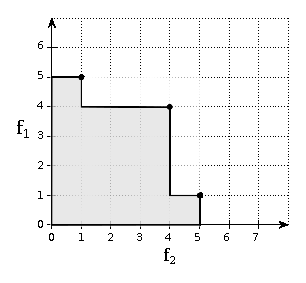
\includegraphics[width=0.5\textwidth]{../img/sce/hypervol2}
  \end{figure}
\end{frame}

\begin{frame}
  \frametitle{Experimentos Computacionais}
  \framesubtitle{Abordagem Heurística}
  Hiper-volume médio alcançado por cada heurística:
  \begin{figure}
    \centering
    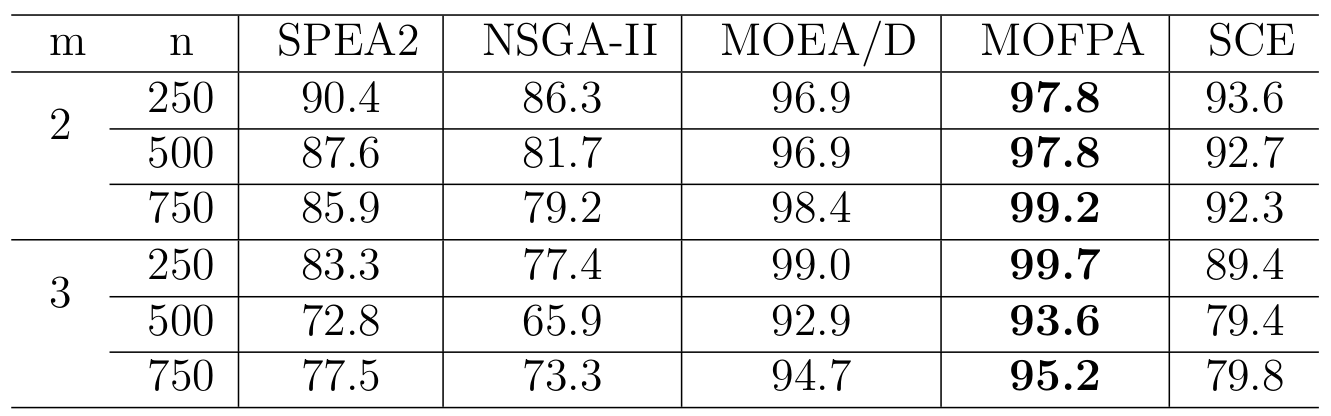
\includegraphics[width=1.0\textwidth]{../tab/sce/zitzler-hvol}
  \end{figure}
\end{frame}

\begin{frame}
  \frametitle{Experimentos Computacionais}
  \framesubtitle{Abordagem Heurística}
  Tempo computacional médio do algoritmo SCE para instâncias Zouache:
  \begin{figure}
    \centering
    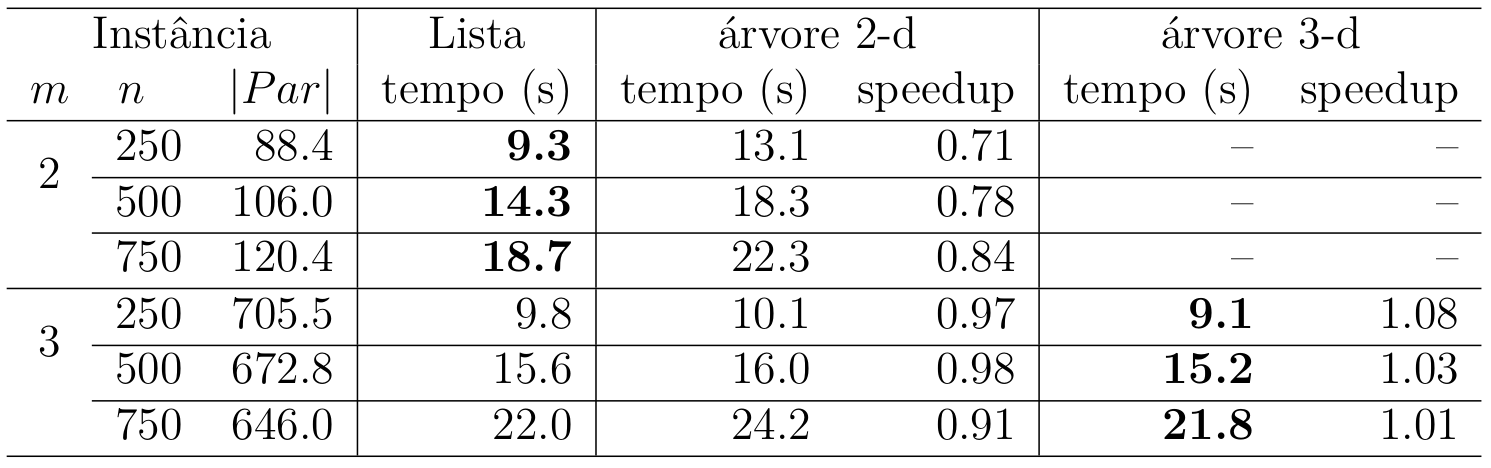
\includegraphics[width=1.0\textwidth]{../tab/sce/cpures}
  \end{figure}
\end{frame}

\begin{frame}
  \frametitle{Experimentos Computacionais}
  \framesubtitle{Abordagem Heurística}
  Número de avaliações médio do algoritmo SCE para instâncias Zouache:
  \begin{figure}
    \centering
    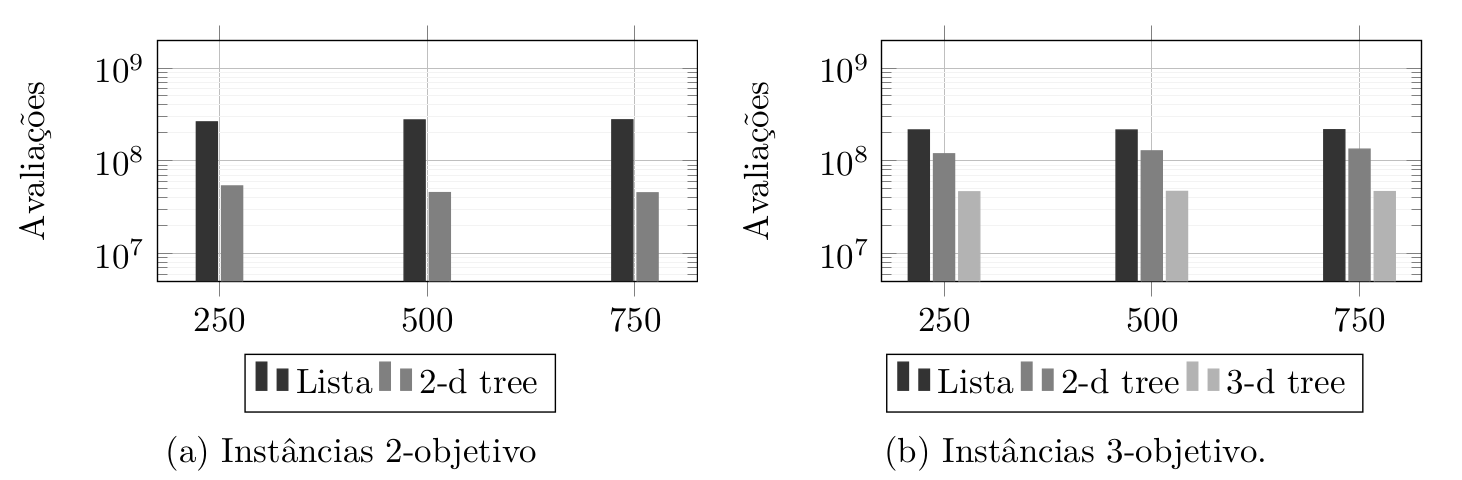
\includegraphics[width=1.0\textwidth]{../tab/sce/cmpres}
  \end{figure}
\end{frame}

\section{Conclusões e Trabalhos Futuros}

\begin{frame}
	\mytitle{Conclusões e Trabalhos Futuros}
\end{frame}

\begin{frame}
	\frametitle{Conclusões}
  \begin{block}{Principais contribuições:}
    \begin{itemize}
      \item{ Interpretação do problema de verificação de dominância como problema de busca de faixa }
      \item{ Proposta da utilização da Árvore KD como estrutura de indexação multidimencional }
      \item{ Análise da proposta em contextos exatos e heurísticos utilizando as principais instâncias da literatura}
    \end{itemize}
  \end{block}
\end{frame}

\begin{frame}
	\frametitle{Conclusões}
  \begin{itemize}
    \item{ Indexação multidimensional foi eficiente no contexto exato: } \pause
    \begin{itemize}
      \item{ Conjuntos solução de alta cardinalidade } \pause
      \item{ Speedup de até $2.3$ para bi-objetivo } \pause
      \item{ Speedup de até $15.5$ para 3-objetivo } \pause
      \item{ Drástica redução no número de avaliações de solução }
    \end{itemize}
    \pause
    \item{ Indexação multidimensional não foi eficiente no contexto heurístico: } \pause
    \begin{itemize}
      \item{ Pouco impacto no tempo computacional } \pause
      \item{ Conjuntos solução de baixa cardinalidade -- overhead } \pause
      \item{ Considerável redução no número de avaliações de solução }
    \end{itemize}
  \end{itemize}
\end{frame}

\begin{frame}
	\frametitle{Tabalhos Futuros}
  \begin{itemize}
    \item{ Verificar a performance da árvore KD em outros problemas
      multiobjetivos;}
    \item{ Considerar outras estruturas de dados
      para auxílio à operação de verificação de dominância;}
    \item{ Aprimorar a implementação do SCE para o MOKP;}
    \item{ Investigar a causa da ineficiência da atual implementação
      do algoritmo Bazgan.}
  \end{itemize}
\end{frame}

\begin{frame}
  \vfill
  \begin{center}
    Obrigado.
  \end{center}
  \vfill
\end{frame}

\begin{frame}
\end{frame}

\end{document}
